%!TEX root = ../main.tex

\section{Measuring the Mössbauer spectrum}
\label{sec:mössbauer-spectrum}

In the following section the Mössbauer spectrum of various materials is measured. The
process of how data is collected and analysed is presented using the example of an 
iron absorber. Other materials are analysed in a similar fashion.

\subsection{Iron}
\label{ssec:iron}

The iron absorber is placed in the beam path. The transmitted photons are counted for
roughly \SI{20}{\minute}. In this measuring mode, the MCS channel number corresponds
to a velocity $v$ at which the $\gamma$-source is moving relative to the iron target.
The 1024 channels available for readout are split into two 512-channel intervals (in the following adressed as Ch1 and Ch2) that differ in the acceleration of the source.
As lined out in the lab manual \autoref{Sch17} it is assumed that the maximum 
velocity $v_\text{max}=\SI{\pm10}{\milli\meter\per\second}$ corresponds to the edges 
of the channel intervals (i.e. Channel \#0 and \#1023 for positive velocity, channel 
\#511, and \#512 for negative velocity). Using this information, a relation between 
channel number $\mathcal{C}$ and $\gamma$-source velocity can be constructed as 
follows:

\begin{equation}
\label{eq:channel-to-velocity}
v(\mathcal{C}) = \SI{10}{\milli\meter\per\second}\cdot\left(\frac{\mathcal{C}-256}{256}\right).
\end{equation}

Because of this relative velocity the photons that are emitted at an energy of 
\SI{14.4}{\kilo\electronvolt} are Doppler shifted to slightly lower/higher energies.
If now a nuclear transition from state $|i\rangle$ to state $|f\rangle$ exists for an
iron atom in the crytal lattice where $E_f-E_i=E'$, there is a nonzero probability 
that the atom absorbs the photon and transitions to the higher energy state. 
Consequently, a dip in the photon spectrum at that specific energy (and by extension 
a specific velocity) can be observed. The resonance around this energy $E'$ can be 
modelled by a slightly modified Breit-Wigner shape presented in \autoref{eq:fitfunc}.

\begin{equation}
\label{eq:fitfunc}
N(E) = \Upphi_0 - \frac{A}{(E-E')^2 - (\frac{1}{2}\,\Gamma)^2},
\end{equation}

where $\Upphi_0$ is the integrated $\gamma$-flux (i.e. number of photons with energy 
$E\approx\SI{14.4}{\kilo\electronvolt}$). The normalisation factor $A$, $E'$ the 
transition energy and $\Gamma$ the full-width-at-half-maximum (FWHM) value of the 
absorption peak. Technically, using this parametrisation of the Breit-Wigner curve, 
$\Gamma$ should also appear in the numerator. To ensure a more stable fit result, 
it has however been absorbed in $A$.

Fitting \autoref{eq:fitfunc} to measurement data, six absorption peaks can be 
identified (see \autoref{fig:iron}). The individual parameters optimised to model
the observed spectrum are listed in \autoref{tab:iron}

\begin{figure}
	\label{fig:iron}
	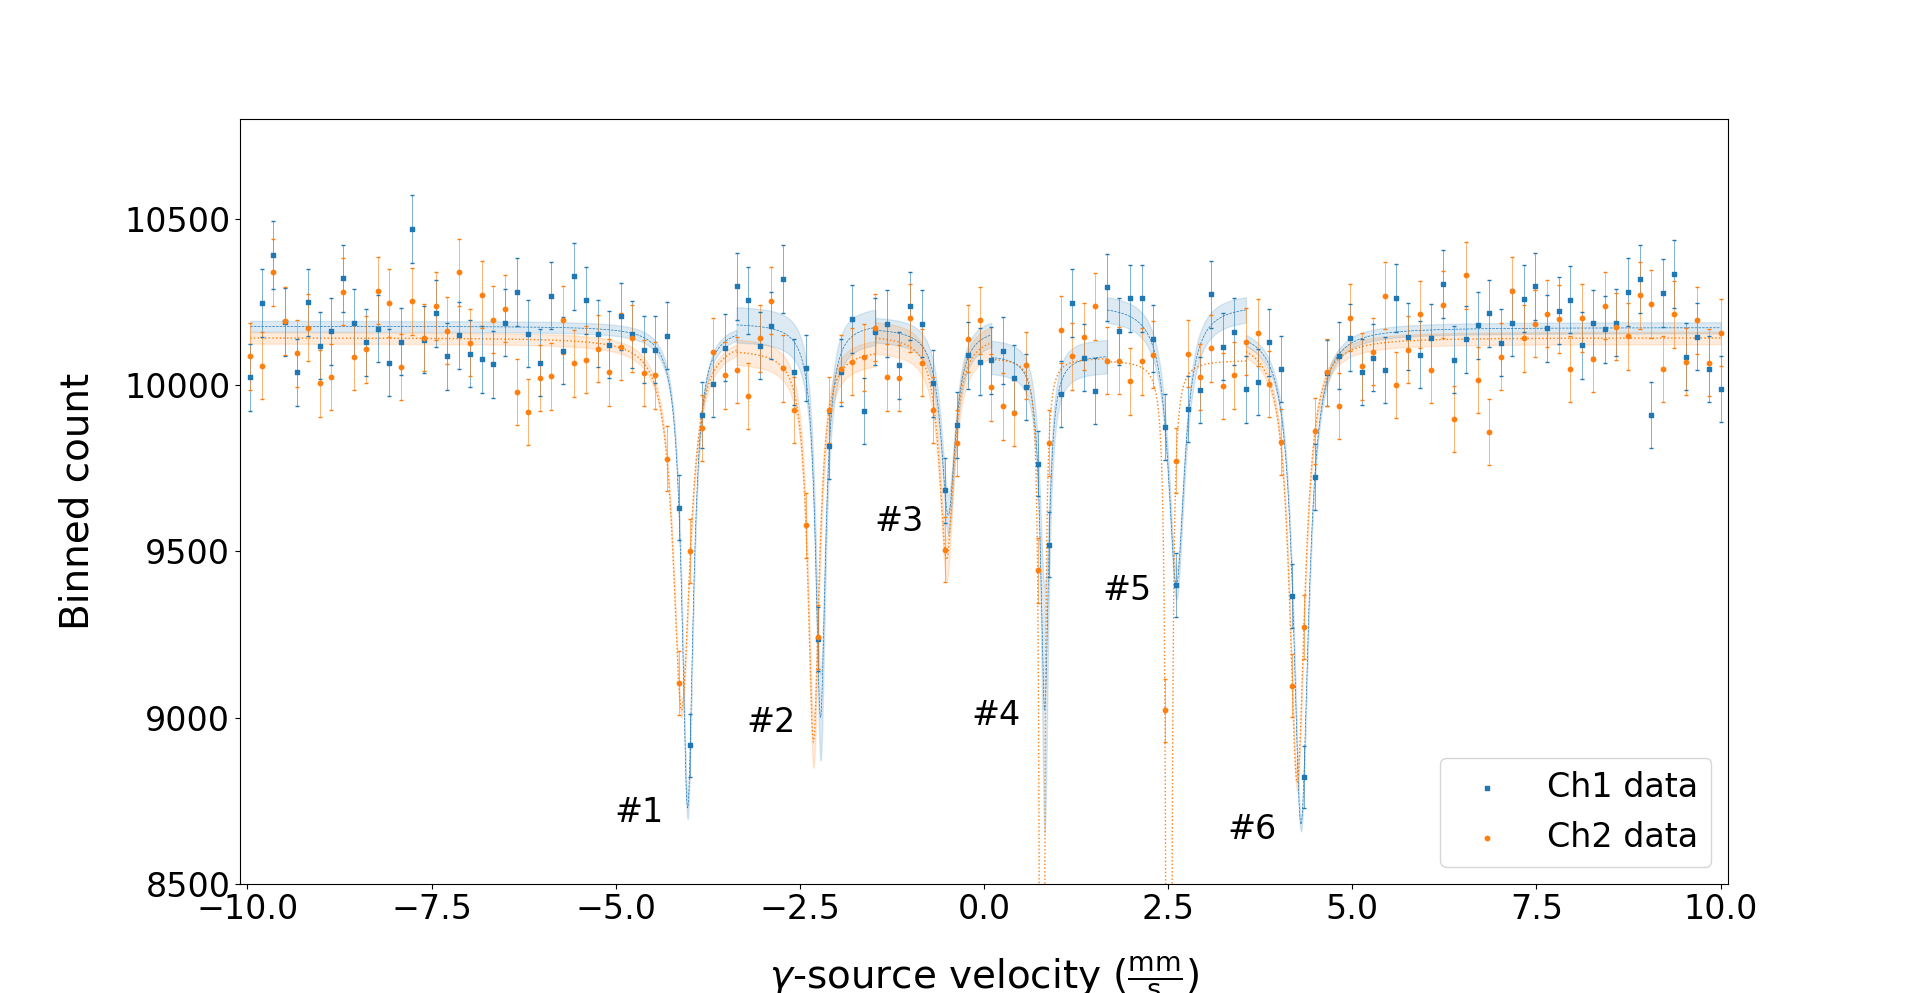
\includegraphics[width=1.0\textwidth]{./fig/Iron.png}
	\caption{Mössbauer spectrum of iron}{CAPTION}
\end{figure}

\todo{Add isometric shift discussion}
